% This file was created by matplotlib2tikz v0.6.15.
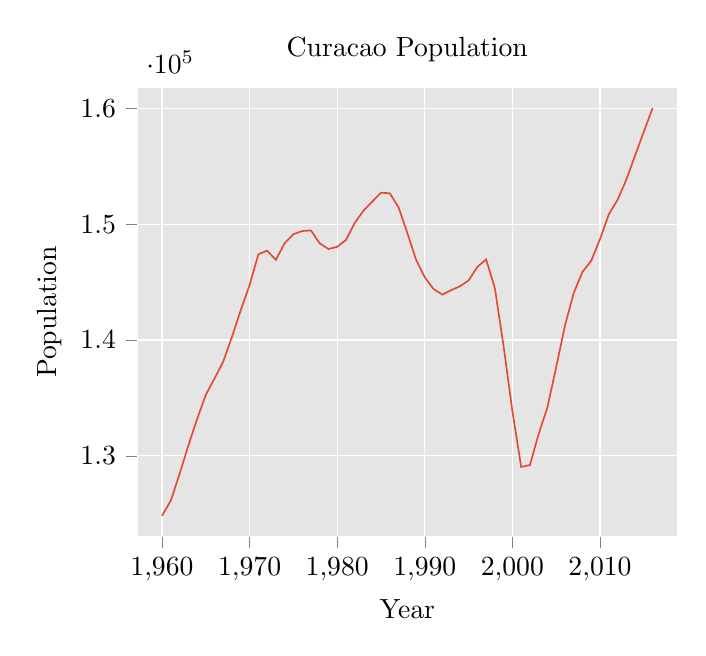
\begin{tikzpicture}

\definecolor{color0}{rgb}{0.886274509803922,0.290196078431373,0.2}

\begin{axis}[
title={Curacao Population},
xlabel={Year},
ylabel={Population},
xmin=1957.2, xmax=2018.8,
ymin=123067.35, ymax=161757.65,
tick align=outside,
tick pos=left,
xmajorgrids,
x grid style={white},
ymajorgrids,
y grid style={white},
axis line style={white},
axis background/.style={fill=white!89.80392156862746!black}
]
\addplot [semithick, color0, forget plot]
table {%
1960 124826
1961 126125
1962 128414
1963 130860
1964 133148
1965 135266
1966 136682
1967 138140
1968 140298
1969 142581
1970 144739
1971 147389
1972 147710
1973 146912
1974 148351
1975 149129
1976 149399
1977 149459
1978 148341
1979 147851
1980 148041
1981 148629
1982 150101
1983 151159
1984 151940
1985 152711
1986 152662
1987 151456
1988 149254
1989 146937
1990 145400
1991 144403
1992 143912
1993 144299
1994 144630
1995 145139
1996 146306
1997 146956
1998 144472
1999 139428
2000 133860
2001 129047
2002 129205
2003 131897
2004 134192
2005 137658
2006 141239
2007 144056
2008 145880
2009 146833
2010 148703
2011 150831
2012 152088
2013 153822
2014 155909
2015 157979
2016 159999
};
\end{axis}

\end{tikzpicture}